\chapter{Introducción}

\section {Motivación}

La criptografía es la técnica mas poderosa en existencia para preservar la privacidad. Un individuo es capaz de proteger información mediante algoritmos y métodos matemáticos de forma que ningún adversario sea capaz de descubrirla, sin importar la cantidad de esfuerzo (o capacidad de cómputo) que este invierta. \\

La importancia de este tipo de tecnologías radica en la protección de un individuo, sus acciones e identidad, en una realidad cada vez más conectada a Internet. \\

En el presente proyecto se ha intentado explorar el alcance de las herramientas y librerías de código libre, tanto en materia de privacidad como anonimato. Y así mismo, la viabilidad de la creación de un software que proteja a sus usuarios, elaborado a manos de un único desarrollador con conocimientos de criptografía, programación e ingeniería del software.

%\emph{ This is a quote }

\section {Tecnologías}
\subsection {Protocolo Signal}
\subsection {The Onion Router}

The Onion Router, también conocido por sus siglas como TOR, es un proyecto de software libre que ha permitido la creación de una red superpuesta a Internet, en la que el tráfico de paquetes se realiza de forma que \hyphenquote{spanish}{imposibilita} descubrir la identidad de los pares que participan en la comunicación. \\

Esto se consigue haciendo que en cada nodo por el que pasan los paquetes estos se cifren sucesivamente, dando lugar a un cifrado por capas donde la información previa sea inaccesible para un nodo intermedio o para alguna entidad maliciosa actuando de \hyphenquote{spanish}{man in the middle}. \\

%TODO: Referencia a "man in the middle".

Los ámbitos de uso de TOR van desde la actividad cotidiana hasta su aplicación para asegurar comunicaciones en zonas de conflicto bélico. También es conocido por sustentar la denominada \hyphenquote{spanish}{Darknet} ó \hyphenquote{spanish}{Deepweb}, cuyo nombre denota las actividades ilícitas que se llevan a cabo bajo el manto de anonimato y privacidad que brinda la tecnología. \\

\begin{figure}[H]
	\centering
	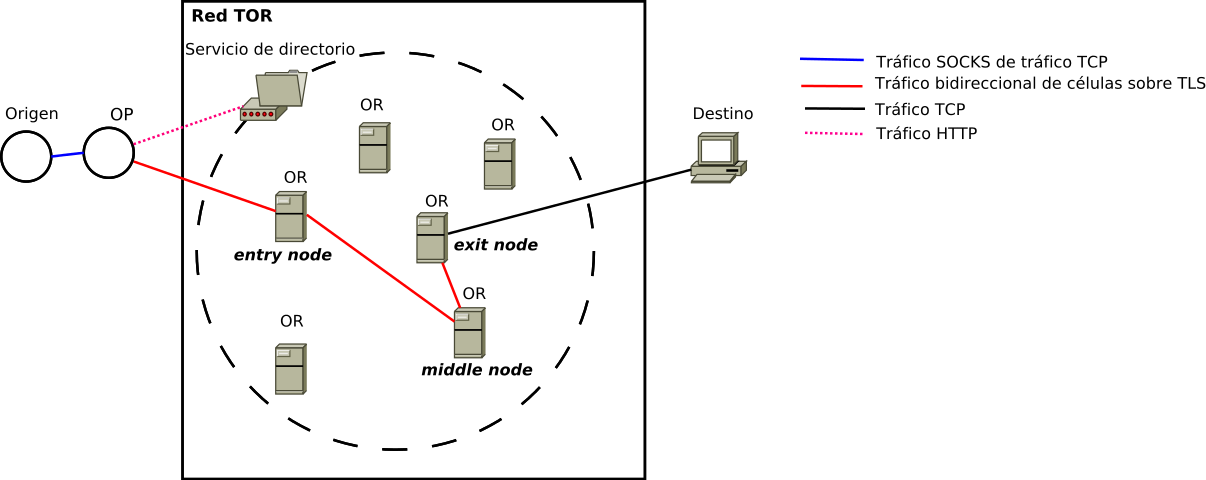
\includegraphics[width=\textwidth]{imagenes/funcionamiento_tor}
	\caption{Funcionamiento de la red Tor.}
	\caption*{\small \url {https://es.wikipedia.org/wiki/Tor_(red_de_anonimato)}}
	\label{fig:redtor}
\end{figure}

\subsubsection {Hidden Services}

Los \hyphenquote{spanish}{hidden services} son, como su nombre indica, servicios alojados en la red TOR que se comunican con sus usuarios de forma exclusiva por medio de la misma. El dominio para acceder a los hidden services se trata de un hash de 16 caracteres derivado de su clave privada y acabado en ``.onion". \\

Los usuarios hacen uso de los \hyphenquote{spanish}{rendezvous points} ó puntos de encuentro (OR que actúan como tales), para conectarse con los hidden services. Es en este punto donde se realiza el intercambio de claves entre usuario y servicio, con el punto de encuentro como intermediario y mediador en la comunicación. \\ 


\subsubsection {Tipos de Nodos}

\textbf {Onion Router (OR)} \\
Entidades clave en la arquitectura de la red, una de sus funciones es enrutar el tráfico a través de la red y actuar como servidores de directorios para la comunicación de los usuarios con hidden services. Los servidores de directorios son OR con operadores de confianza, encargados de mantener y difundir la base de datos con la información de otros OR. \\

Cuando un OR se conecta a la red, se define a sí mismo compartiendo y exponiendo su funcionamiento y capacidades (versión, banda ancha, política de enrutamiento, etc). \\

\textbf {Onion Proxy (OP)} \\
Se trata de la entidad que representa el software ejecutado por el usuario. Obtiene además información acerca del estado de la red y realiza el cálculo del camino aleatorio de la comunicación. De forma que pueda cumplir su función de enrutar el tráfico TCP hacia TOR.

\subsubsection {Funcionamiento}

Las aplicaciones que deseen comunicarse mediante TOR pueden hacerlo siguiendo la interfaz SOCKS, la cual actúa como intermediaria entre la aplicación y la red. \\

Una vez conectado a la red, el usuario solicita a un servicio de directorio información sobre la red (Nodos OR), y decide un camino aleatorio para los paquetes. Este camino consta de un nodo de entrada, un nodo intermedio y un nodo de salida. \\

El camino de la comunicación se genera de forma sucesiva: primero generando las claves de cifrado, posteriormente aplicando un \hyphenquote{spanish}{Diffie-Hellman} entre los puntos a comunicarse y por último el envío de las claves y comunicación cifrada mediante \hyphenquote{spanish}{RSA} (claves pública y privada). \\

%TODO: Referencias a Diffie-Helman y a RSA.

Una vez que las claves RSA han sido establecidas, este es considerado como un medio seguro para la comunicación, y se procede al envío de los paquetes que irán encapsulados en capas de cifrado que se podrán romper a cada salto hasta llegar al destino. \\ 

%TODO: Refrasear lo ultimo, lo de los saltos.

\begin{figure}[H]
	\centering
	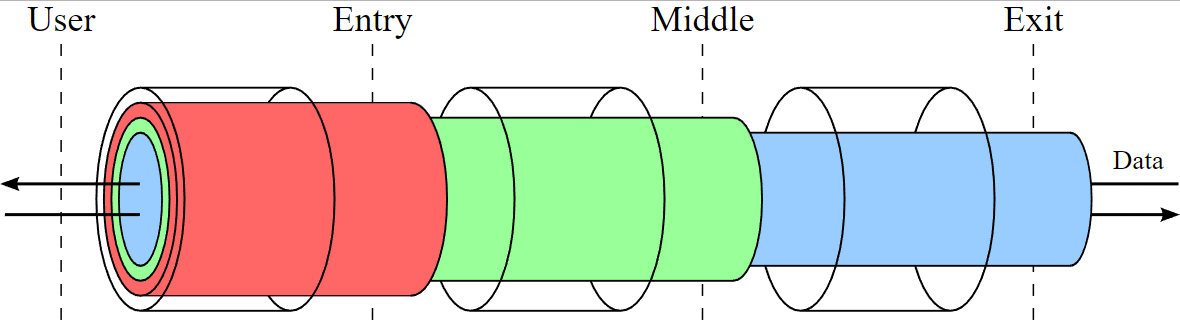
\includegraphics[width=\textwidth]{imagenes/tor_keys}
	\caption{Funcionamiento de la red Tor.}
	\caption*{\small \url {https://svn.torproject.org/svn/projects/presentations/security-part2-anon/}}
	\label{fig:torkeys}
\end{figure}

\subsubsection {Puntos flacos}

Pese a disponer de un extenso equipo de expertos desarrolladores y criptógrafos, TOR está sujeto a una constante caza de vulnerabilidades y búsqueda de métodos para romper la protección que brinda a los usuarios. \\
Los principales interesados en conseguirlo son entidades gubernamentales y servicios de inteligencia de diversos países, que pese a esto, son también usuarios de primera mano de TOR y sus servicios. \\ 

Los principales ataques se basan en la correlación de tiempos de envío y tamaños de paquetes en la red, los cuales mediante una análisis sistemático y controlando un relativamente grande numero de nodos, permitirían destapar la identidad de los usuarios. \\

Desde un punto de vista de usuario, la principal desventaja de TOR se halla en que por diseño, su característica es la protección de la identidad de la cual proviene la información, pero no la ofuscación o privacidad de la misma. Es decir, pese a usarse la red TOR para acceder a un servicio, si la comunicación se realiza en texto plano, cualquier tercero escuchando tanto en la entrada o salida de la red podrá interceptar las comunicaciones. \\ 

Los puntos principales que podrían comprometer nuestra identidad durante su uso son los siguientes: \\

\begin{itemize}  
	\item  Código Javascript malicioso
	\item  Cookies
	\item  Cabeceras HTTP
	\item  Uso de HTTP en lugar de HTTPS
	\item Peticiones DNS no redireccionadas por TOR
	\item  Plugins (Java, Flash, etc)
\end{itemize}

\subsection {Node.js}

Node.js es un interprete de JavaScript desarrollado sobre el motor V8 de Chrome, de forma que extiende el uso del lenguaje también en el lado del servidor. Consta además, de uno de los ecosistemas de librerías más grandes en existencia. \\

Pese a disponer de una librería para el manejo de operaciones sobre HTTP, es también gracias a paquetes como Express o Hapi que Node.js se ha extendido en gran medida como herramienta para desarrollar servidores y aplicaciones web. \\
El modelo de Node.js esta basado en eventos y operaciones de E/S no bloqueantes, lo que lo hace eficiente en el tratamiento de peticiones concurrentes.

\subsection {Websockets}

Websocket es un protocolo que propociona un canal de comunicación bidireccional entre cliente y servidor sobre un mismo socket TCP. \\

El uso de sesiones de este tipo es especialmente útil en aplicaciones donde es ventajoso que el servidor pueda enviar datos también al cliente; siendo este caso imposible en las formas de comunicación convencionales entre cliente y servidor como XHR (AJAX), donde es el cliente el encargado de iniciar cada intercambio de información. \\

El protocolo de websockets consta de soporte en las versiones más modernas de casi todos los navegadores. Sin embargo, puede no ser viable su uso en versiones más antiguas. Para solventar este problema, se ha hecho uso de la librería Socket.io de Node.js. \\

Socket.io implementa una interfaz para la comunicación sobre websockets con un mecanismo para pivotar hacia otros modelos de comunicación en caso de que el medio no conste de soporte para estos. \\
\subsection {Electron}

Electron es una librería desarrollada por Github que permite crear aplicaciones de escritorio multiplataforma mediante Javascript, CSS y HTML. \\
Ésto se consigue combinando Node.js y Chromium (navegador de código libre sobre el que está basado Chrome). De esta forma se crea un entorno de ejecución con funcionalidades cliente-servidor. \\

Una de las principales aplicaciones desarrolladas con Electron es Atom, el editor de texto de código libre desarrollado por Github. Sin embargo, hay multitud de aplicaciones utilizadas por millones de usuarios que se apoyan en esta tecnología, entre ellas encontramos Slack, Visual Studio Code, Wordpress.com y Discord, entre otras. \\

\subsection {React}

React es una librería desarrollada por Facebook para la creación de interfaces de usuario basadas en componentes. \\

Hace uso de JSX, una sintaxis extendida de Javascript que permite la declaración de etiquetas HTML junto con variables y funciones, además de otras características. \\

Los componentes se suelen organizar de forma jerárquica, donde la información fluye del componente padre a sus hijos, en forma de propiedades (props). Los componentes hijos tienen la capacidad de notificar al padre de una acción de usuario o un cambio de estado mediante llamadas a funciones (recibidas en forma de props).\\

\subsubsection {Componentes, estado, propiedades y renderizado}

Los componentes constan de estado, propiedades y ciclo de vida. El estado son las características propias del componente, mientras que las propiedades son aquellos valores recibidos externamente, normalmente por el componente padre. Al cargarse la vista, estos se renderizan, y conforme el estado se modifica por acciones del usuario o las propiedades recibidas cambian, estos avanzan por las distintas etapas del ciclo de vida y vuelven a renderizarse. \\

\subsubsection {DOM Virtual}

React genera un DOM virtual sobre el que se construyen los componentes. Después de una actualización del estado se compara el DOM anterior con el actual, actualizando y modificando de forma eficiente la vista, ya que solo se renderizan de nuevo aquellas partes necesarias.  \\

\subsubsection {Multiplataforma}

Facebook ha desarrollado también una adaptación de React para plataformas móviles, llamada React Native.

\subsection {React Native} 

Ésta funciona con los mismos principios que React y también se desarrolla mediante Javascript, pero utilizando en el renderizado componentes propios de la librería en lugar de etiquetas HTML, que posteriormente se traducen a componentes nativos. De esta forma es posible creat una aplicación móvil nativa y con todas las propiedades de las mismas. \\

\subsection {Redux}

Redux es una librería de Javascript, que aunque agnóstica, ha sido desarrollada con su uso combinado con React en mente. \\ 

Redux permite mantener un estado central de la aplicación como única fuente de verdad e implementa un flujo de información unidireccional, que resulta muy ventajoso en aplicaciones grandes y/o complejas. \\

El proceso de actualización de estado en Redux es el siguiente: 

\begin{enumerate}  
	\item  Un evento, por ejemplo la interacción del usuario, produce un cambio en la vista.
	\item Se despacha una acción asociada a ese evento. 
	\item La acción es procesada por un \hyphenquote{spanish}{reducer}, que se encarga de interpretar esa acción y aplicar el cambio sobre la \hyphenquote{spanish}{Store}, o el estado central de la aplicación, conforme corresponda.
\end{enumerate}

Para operaciones asíncronas, como llamadas a APIs o eventos similares, Redux puede emplearse con middlewares que extienden su funcionalidad. Para este caso tenemos \hyphenquote{spanish}{redux-thunk}, que permite declarar acciones más allá de simple objectos Javascript, y declararlas como funciones. De esta manera pueden lanzarse diversas acciones dependiendo del estado de la petición o la operación, manteniendo la \hyphenquote{spanish}{Store} actualizada en todo momento. \\

Las acciones se ejecutan de forma secuencial, evitando de esta manera condiciones de carrera o estados inconsistentes de los datos. \\

\subsubsection {Estado inmutable}

La \hyphenquote{spanish}{Store}, o el estado de la aplicación, se trata de un objeto que contiene toda la información referente a esta y se trata de forma inmutable. O lo que es lo mismo, cuando se debe actualizar el estado de la aplicación debido a una acción, los \hyphenquote{spanish}{reducers} crean una copia del estado anterior modificado, y este substituye al estado anterior. Esto resulta de especialmente eficiente cuando se deben tratar gran cantidad de datos con cambios constantes o sistemáticos. Resulta mucho más rápido que la comparación en más profundidad. \\

Para realizar estas operaciones se hace uso de librerias que tratan los objectos como inmutables, de la función Object.assign(...) ó si se dispone de la versión de Javascript ES6 en el proyecto, el operador \hyphenquote{spanish}{spread}. \\

